\documentclass[a4paper,twoside,11pt]{report}
\usepackage{geometry}
\usepackage{fullpage}
\usepackage[czech]{babel}
\usepackage[utf8]{inputenc}
\usepackage[T1]{fontenc}
\usepackage{hyperref}
\usepackage{microtype}
\usepackage{listings}
\usepackage{lmodern}
\usepackage{marginnote}
\usepackage{syntax}
\usepackage{at}
\usepackage{makeidx}
\usepackage{graphicx}
\usepackage{float}
\usepackage{caption}
\usepackage{subcaption}
\usepackage[fixlanguage]{babelbib}
\usepackage{tabularx}
\usepackage{changepage}
\usepackage{tikz}
\usetikzlibrary{positioning}
\usetikzlibrary{calc}

\geometry{
  marginparsep=0.3cm,marginparwidth=1.5cm,
  inner=2.5cm,outer=3.0cm,
  top=2cm,bottom=2cm,
}

\selectbiblanguage{czech}

\lstloadlanguages{Haskell}

\lstdefinestyle{haskell}{
  basicstyle=\small\ttfamily,
  flexiblecolumns=false,
  basewidth=0.5em,
  language=Haskell,
  showstringspaces=false,
  keywords={ % use only real Haskell keywords
    case,class,data,default,deriving,do,else
    ,foreign,if,import,in,infix,infixl
    ,infixr,instance,let,module,newtype,of
    ,then,type,where
  },
  otherkeywords={_},
  texcl=true,
}

% code chunks in literate haskell
\lstnewenvironment{code}[1][]{\lstset{style=haskell,#1}}{}
% code chunks which should NOT be processed by literate haskell
\lstnewenvironment{haskell}[1][]{\lstset{style=haskell,#1}}{}

\lstdefinestyle{krunimir}{
  basicstyle=\small\ttfamily,
  flexiblecolumns=false,
  basewidth=0.5em,
  keywords={
    forward,left,right,color,pen,split,if,repeat,define
  },
}

\DisableLigatures[>,<]{encoding = T1,family=tt*} %

\setlength{\grammarparsep}{5pt plus 1pt minus 1pt} 
\setlength{\grammarindent}{12em}

\renewcommand*{\marginfont}{\scriptsize}

\newcommand{\comment}[1]{}
\newatcommand t[1]{\texttt{#1}}

\makeindex
\newatcommand idx[1]{\index{#1@\texttt{#1}}}
\newatcommand Idx[1]{\index{#1@\texttt{#1}|textbf}}

\def\Cplusplus{{C\nolinebreak[4]\hspace{-.05em}\raisebox{.4ex}{\tiny\bf ++}}}
\def\Csh{C\nolinebreak\hspace{-.05em}\raisebox{.4ex}{\scriptsize\bf \#}}

\hypersetup{
  unicode=true,          % non-Latin characters in Acrobat’s bookmarks
  pdftitle={Líně, čistě, funkcionálně},    % title
  pdfauthor={Jan Špaček},     % author
  hidelinks,
  % hyperindex should be true by default, hyperref shows warning 
  % "Option `hyperindex' has already been used,"
  % hyperindex=true,
  linktoc=all,
}

\begin{document}
%%% The halftitle

\begin{titlepage}
\begin{center}

\textsc{\LARGE Středoškolská odborná činnost}\\[4cm]

\textsc{\Huge Líně, čistě,\\ funkcionálně}

\textit{\large aneb}

\textit{\LARGE Užití funkcionálního programovacího jazyka Haskell k řešení
úloh Ústředního kola ČR Soutěže v programování}\\[2cm]

\textsc{\huge Jan Špaček}\\[10cm]

\textit{\LARGE Ostrava 2013}

\end{center}
\end{titlepage}

% hides the page number
\thispagestyle{empty}
\cleardoublepage

%%% The title

\begin{center}

\textsc{\LARGE Středoškolská odborná činnost}\\[0.6cm]
\textsc{\large Obor SOČ: 18 Informatika}\\[2cm]

\textsc{\Huge Líně, čistě,\\ funkcionálně}

\textit{\large aneb}

\textit{\LARGE Užití funkcionálního programovacího jazyka Haskell k řešení
úloh Ústředního kola ČR Soutěže v programování}\\[2cm]

\textsc{\huge Lazy, pure, functional}

\textit{\Large Using the functional programming language Haskell to solve
tasks from the finals of the Czech Programming Contest}\\[3cm]

\begin{tabularx}{12cm}{
  >{\Large\scshape}p{3cm} 
  >{\LARGE}X 
}
Autor:    & Jan Špaček \\[0.5cm]
% aww, how dirty! :)
Škola:    & Wichterlovo gymnázium \\[0.15cm]
          & Čs.~exilu 669 \\[0.2cm]
          & Ostrava-Poruba \\
\end{tabularx}
\\[3cm]

\textit{\LARGE Ostrava 2013}

\end{center}

\setcounter{page}{1}
\thispagestyle{empty}

\newpage

%%% The declaration

~\\[15cm]
\section*{Prohlášení}

Prohlašuji, že jsem svou práci vypracoval(a) samostatně, použil(a) jsem pouze
podklady (literaturu, SW atd.) uvedené v přiloženém seznamu a postup při
zpracování a dalším nakládání s prací je v souladu se zákonem č. 121/2000 Sb.,
o právu autorském, o právech souvisejících s právem autorským a o změně
některých zákonů (autorský zákon) v platném znění.\\[0.5cm]

V \makebox[3cm]{\dotfill} dne \makebox[4cm]{\dotfill}
podpis: \makebox[6cm]{\dotfill}

\newpage

%%% Thanks

~\\[15cm]
\textit{
Nejen ve své práci jsem využil nepřeberného množství svobodného softwaru.
Zvláště bych rád poděkoval autorům těchto projektů:
GNU/Linux (svobodný operační systém),
Ubuntu a jeho odnož Xubuntu (linuxové distribuce),
Vim (textový editor),
Git (distribuovaný systém správy verzí),
\LaTeX\ (sázecí systém),
Haskell (jazyk, kolem kterého se v této práci všechno točí),
GHC (špičkový překladač Haskellu).
}

\newpage

\begin{adjustwidth}{1.5cm}{1.5cm}

% there is a copy of this abstract in README which must be kept in sync!

\section*{Abstrakt}

Funkcionální programování, vycházející z $\lambda$-kalkulu, tvoří alternativu k
dnes široce využívanému imperativnímu přístupu k programování, reprezentovanému
jazyky jako C, \Cplusplus{}, Java, \Csh{}, Objective-C, JavaScript, Python, Ruby
či PHP.

Tyto jazyky jsou založeny na postupném vykonávání příkazů, jež mění stav
programu (zvláště hodnoty proměnných). Naproti tomu funkcionální jazyky provádí
výpočty vyhodnocováním výrazů. Základní stavební prvky -- funkce -- jsou od
imperativních protějšků (ať už procedur, metod nebo \uv{funkcí} jako v jazyce C)
odlišné tím, že jejich výsledek vždy závisí pouze na vstupních argumentech, čímž
se přibližují matematickým funkcím.

Algoritmy zapsané ve funkcionálním jazyce tudíž nemají podobu série kroků, jež
se musí postupně vykonat a jež určují \emph{jak} se k výsledku dostat, ale spíše
popisují \emph{co} je jejich výsledkem.

V této práci je představeno řešení dvou úloh Ústředního kola ČR Soutěže v
programování z let 2010 a 2012 užitím funkcionálního programovacího jazyka
Haskell. Cílem je čtenáře seznámit s vysokoúrovňovými koncepty, které se ve
funkcionálních programech používají, a jejich aplikací při řešení
\uv{skutečných} úloh.

\paragraph*{Klíčová slova}
Funkcionální programování; Haskell; želví grafika; AI.

\section*{Abstract}

Functional programming, rooted in $\lambda$-calculus, is an alternative to the
mainstream imperative approach to programming, as seen in languages like C,
\Cplusplus{}, Java, \Csh{}, Objective-C, JavaScript, Python, Ruby či PHP.

These languages are based on statements, which are sequentially executed and
change the program's state. In contrast, functional languages treat computations
as evaluation of expressions. The fundamental way in which basic building blocks
of functional languages -- functions -- differ from their imperative
counterparts (procedures, methods or C-style ``functions'') is that their result
depends entirely on their arguments. This makes the functions used in
programming much closer to functions used in mathematics.

Algorithms in a functional language are not a sequence of steps describing
\emph{how} the result should be computed, but they rather specify \emph{what}
the result is.

In this paper, we present a solution to two tasks from the final of The Czech
Programming Contest held in 2010 and 2012, using the functional programming
language Haskell. The goal of the paper is to make the reader familiar with the
high-level concepts used in functional programs and their usage in solving
``real'' problems.


\paragraph*{Keywords}
Functional programming; Haskell; turtle graphics; AI.

\end{adjustwidth}

\tableofcontents
\chapter{Úvod}

\section{Co je to Haskell}

Haskell je \textit{de-facto} standardní líný čistě funkcionální jazyk. Jeho
vývoj začal v září roku 1987, přičemž první verze jazyka (Haskell 1.0) byla
vydána 1. března 1990. Postupně následovaly verze 1.1 až 1.4. V roce 1999 byla
vytvořena \uv{stabilní} verze Haskell 98\comment{cite Haskell 98 Report}, která
byla později revidována.\comment{cite Haskell 98 Revised Report}

\marginnote{Citace, citace, citace!}

Od roku 2006 probíhá proces nazývaný Haskell' (Haskell Prime), jehož cílem je
vytvářet nové revize standardu každý rok. První a zatím poslední revizí je
Haskell 2010.\comment{cite Haskell 2010 Report}

\marginnote{úvodní odstavec k vlastnostem}

\subsection{Čistě funkcionální}

V \emph{imperativních} programovacích jazycích (C, C++, Java, Ruby, JavaScript,
Befunge, PHP...) jsou algoritmy vyjádřeny jako sekvence kroků -- příkazů, které
mění stav programu, zvláště hodnoty proměnných.  Tento přístup přímo vychází ze
strojového kódu počítačů a v dnešní době jde o dominantní programovací styl.

\emph{Funkcionální} jazyky jsou oproti tomu založeny na vyhodnocování výrazů a
jejich fundamentálním typem je \emph{funkce}. Narozdíl od imperativních jazyků,
kde vyhodnocování výrazů a volání procedur (metod) může mít \emph{vedlejší
účinky}, např. změnu hodnoty proměnných nebo vypsání řetězce na obrazovku,
jediný účinek, který má \uv{zavolání} (aplikace) funkce ve funkcionálním jazyku,
je získání jejího výsledku. Jelikož neexistuje žádný stav, na němž by výsledek
funkce mohl záviset, je garantováno, že aplikujeme-li funkci vícekrát na stejné
argumenty, dostaneme vždy stejný výsledek. Tato vlastnost se nazývá
\emph{referenční transparentnost}.

Na funkce je tedy možno nahlížet jako na funkce v matematice, takže pro
programátora i pro kompilátor je snadné zjišťovat a \emph{dokazovat} chování
funkce.

\marginnote{velmi snadná paralelizace!}

\subsection{Líně vyhodnocovaný}

\emph{Líné vyhodnocování} znamená, že hodnoty výrazů se počítají až ve chvíli,
kdy je to nezbytně nutné. Tím se nejen zvýší efektivita programu (výpočty se
provedou jen když jsou zapotřebí, nemusí se tedy vyhodnotit vůbec), ale hlavně
se programátor zbaví nutnosti zabývat se pořadím vyhodnocování výrazů. Je tedy možné
oddělit kód produkující a kód konzumující data, čímž se zvýší modularita. 

\marginnote{citovat Why FP Matters}

Ve funkcionálních programech je běžné používat nekonečné struktury, např.
nekonečné seznamy či nekonečně se větvící stromy, a nechat vyhodnotit pouze tu
část dat, která je potřeba k získání požadovaného výsledku.

\subsection{Staticky typovaný}

\emph{Statické typování} znamená, že typ každého výrazu je znám již v při
kompilaci programu, takže případné chyby kompilátor odhalí velmi brzy. Není tedy
možné, aby program za běhu zhavaroval na typovou chybu, čímž se eliminuje celá
škála potencionálních bugů -- žádné @t{Segmentation fault}, žádné
@t{NullPointerException}, žádné @t{NoMethodError}. Většinou platí, že když se
kód úspěšně zkompiluje, máme velkou šanci, že bude skutečně fungovat tak, jak si
představujeme.

Narozdíl od jazyků jako Java či C++, jež jsou také staticky typované, je silný
typový systém Haskellu schopen naprostou většinu typů odvodit sám, takže typové
anotace se obvykle používají jako druh dokumentace určené hlavně pro člověka.

\subsection{Typové třídy}

S typovým systémem úzce souvisí \emph{typové třídy}.\footnote{Neplést s třídami
z objektově orientovaných jazyků} Typové třídy byly do Haskellu zavedeny, aby se
vyřešil problém s \uv{přetěžováním} funkcí jako je porovnávání (@t{==}), které
bychom potřebovali použít s větším množstvím typů (operace ekvivalence má smysl
např. pro čísla, řetězce, seznamy, množiny...).

Ukažme si příklad typové třídy @t{Eq}, která slouží k implementaci porovnání
dvou hodnot:

\begin{haskell}
class Eq a where
  (==) :: a -> a -> Bool
\end{haskell}

Tímto deklarujeme, že typ @t{a} patří do třídy @t{Eq} právě tehdy, když
implementuje metodu @t{==}.

Mějme dva datové typy:

\begin{haskell}
data Color = Red | Green | Blue
data Bit = On | Off
\end{haskell}

Pro oba tyto typy určitě dává operace porovnání smysl, proto můžeme nadefinovat
\emph{instanci} třídy @t{Eq}:

\begin{haskell}
instance Eq Color where
  Red   == Red   = True
  Green == Green = True
  Blue  == Blue  = True
  _ == _ = False

instance Eq Bit where
  On  == On  = True
  Off == Off = True
  _   == _   = False
\end{haskell}

Touto deklarací specifikujeme, že typy @t{Color} a @t{Bit} jsou instancemi třídy @t{Eq}, a
poskytneme implementaci metody @t{==}. Nyní můžeme používat funkci @t{==} s
barvami i bity, např. @t{Red == Red} vrátí @t{True} a @t{On == Off} vrátí
@t{False}.

Všimněte si, že nemůžeme porovnávat barvy a bity -- napíšeme-li @t{Red == On},
kompilátor vyhodí typovou chybu, jelikož funkce @t{==} akceptuje pouze hodnoty
stejného typu.

Kdybychom chtěli funkci, která otestuje, jestli se daný prvek nachází v
seznamu, mohli bychom si ji nadefinovat takto:

\begin{haskell}
elem :: Eq a => a -> [a] -> Bool
elem _ [] = False
elem x (y:ys) = if x == y then True else elem x ys
\end{haskell}

Typ této funkce, @t{Eq a => a -> [a] -> Bool}, odráží skutečnost, že tato funkce
je definovaná pouze pro takové typy @t{a}, které náleží do třídy @t{Eq}. Můžeme
ji tedy použít jak na seznam barev (@t{[Color]}), tak na seznam bitů
(@t{[Bit]}).

Instancemi tříd samozřejmě nemusí být jen takového jednoduché typy.  Můžeme si
nadefinovat typ reprezentující binární strom:

\begin{haskell}
data Tree a = Node (Tree a) (Tree a) | Leaf a
\end{haskell}

Tento typ bychom obratem mohli učinit instancí třídy @t{Eq}:

\begin{haskell}
instance Eq a => Eq (Tree a) where
  Leaf x == Leaf y         = x == y
  Node l1 r1 == Node l2 r2 = l1 == l2 && r1 == r2
  _ == _ = False
\end{haskell}

Tato instance deklaruje, že pro všechny typy @t{a} je typ @t{Tree a} instancí
třídy @t{Eq}, platí-li, že typ @t{a} je rovněž instancí @t{Eq}.

\chapter{Krunimír: želví grafika}

\begin{quotation}

Želvák Krunimír je velký myslitel. Zjistil, ze když si za krunýř přiváže trochu
křídy, kreslí za sebou při svém plazení cestičku. I pojal plán nakreslit svoji
podobiznu, samozřejmě včetně přesných detailů krunýře. Hned se dal pln nadšení
do díla a práce mu šla pěkně od ... tlapy.

\uv{Co to děláš, dědečku,} zeptal se jednou Krunimíra jeho vnuk Krunoslav.
\uv{Krešlím tady švou poďobižnu,} odpověděl Krunimír. \uv{Žačal jsem š ní, když
tvůj tatík ještě nebyl na švětě, a ještě nemám ani krunýř,} dodal smutně. \uv{To
už ji aši dokrešlit neštihnu...}  Vnuk Krunoslav, znalec moderní techniky, mu
však poradil: \uv{Tak si nech napsat program, který ji nakreslí za Tebe.}
Protože se ale s tlapami a zobákem moc dobře neprogramuje, najali si želváci
vás.

\end{quotation}

Takto začíná zadání finální úlohy Soutěže v programování z roku 2010. Popisuje
jednoduchý procedurální jazyk na generování želví grafiky, inspirovaný jazykem
Logo, a úkolem je vytvořit interpret tohoto jazyka, jehož vstupem je text
programu a výstupem vykreslený obrázek.

\marginnote{Hodil by se nějaký popsaný obrázek s výsledkem Krunimírovy práce,
třeba některý ze stromů.}

\section{Popis jazyka}

Uživatel má k dispozici několik primitivních kreslících funkcí:

\begin{description}
\item[@t{forward(d)}] Želva se posune vpřed o @t{d} jednotek (pixelů).
Pokud je tloušťka pera kladná, zanechá za sebou čáru vedoucí z původní pozice do
nové. Takovýto pohyb se považuje za jeden \emph{tah}.
\item[@t{right(a)}, @t{left(a)}] Želva se otočí doprava, resp. doleva o
@t{a} stupňů.
\item[@t{pen(s)}] Nastaví tloušťku pera na @t{s}
\item[@t{color(r, g, b)}] Nastaví barvu pera, @t{r}, @t{g} a
@t{b} jsou jednotlivé složky modelu RGB v rozsahu 0 až 255.
\end{description}

Jazyk dále umožňuje použít jednoduchou podmínku a cyklus:

\begin{description}
\item[@t{if(x) \{ ... \}}] Vykoná příkazy v těle podmínky právě když je
@t{x} kladné.
\item[@t{repeat(x) \{ ... \}}] Vykoná příkazy @t{x}-krát, je-li
@t{x} kladné.
\end{description}

Uživatel může definovat vlastní procedury a volat je:

\begin{description}

\item[@t{define 
  \textit{procedura}(\textit{p1},\textit{p2},...)
  \{ ... \}
}]
  Definuje proceduru \textit{procedura}, která má libovolný počet parametrů
  (\textit{p1}, \textit{p2}, ...). Tyto parametry mohou být v těle procedury
  použity ve výrazech a nabývají hodnoty předané v místě volání.

\item[@t{\textit{procedura}(\textit{arg1},\textit{arg2},...)}]
  Zavolá proceduru \textit{procedura} s argumenty (\textit{arg1}, \textit{arg2},
  ...). Procedura musí být definována \textit{před} svým voláním a může být
  rekurzivní.

\end{description}

Poslední a nejzajímavější struktura je rozdvojení:

\begin{description}
\item[@t{split \{ ... \}}] Vytvoří klon aktuální želvy, která vykoná
příkazy v těle struktury @t{split}, přičemž původní želva pokračuje ve vykonávání
dalších příkazů. Všechny želvy se pohybují paralelně, vždy všechny provedou
jeden \emph{krok}, poté druhý atd.
\end{description}

Jako argumenty při volání procedur lze používat výrazy vytvořené z celočíselných
literálů, parametrů aktuální procedury, binárních operátorů @t{+}, @t{-},
@t{*} a @t{/} (celočíselné dělení) a negace pomocí operátoru
@t{-}. Ve výrazech je možno používat závorky @t{(} a @t{)},
priorita a asociativita operátorů je jako v matematice.

\subsection{Příklady}

Výstupy těchto příkladů jsou na obrázku \ref{fig:krunimir-examples}.

\subsubsection{Čtverec (\ref{fig:krunimir-square1})}

Jednoduchý kód, který vykreslí čtverec. 
\lstinputlisting[style=krunimir]{krunimir/examples/square1.txt}

\subsubsection{Mřížka čtverců (\ref{fig:krunimir-squares})}

V této ukázce využijeme procedury, abychom kód rozdělili na menší a přehlednější
části.
\lstinputlisting[style=krunimir]{krunimir/examples/squares.txt}

\subsubsection{Binární strom (\ref{fig:krunimir-bintree})}

Při vykreslování stromů prokáže svoji užitečnost příkaz @t{split}.
\lstinputlisting[style=krunimir]{krunimir/examples/bintree.txt}

% příklady a jejich výsledky by opravdu neměly utéct někam pryč, proto H
\begin{figure}[H]
  \centering

  \begin{subfigure}{0.3\textwidth}
    \centering
    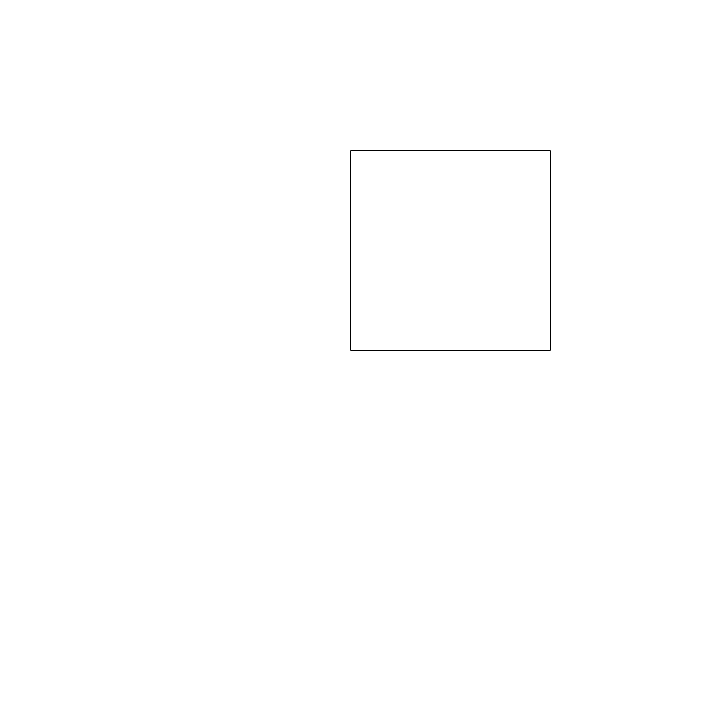
\includegraphics[width=\textwidth]{krunimir/examples/square1}
    \caption{Čtverec}\label{fig:krunimir-square1}
  \end{subfigure}
  ~
  \begin{subfigure}{0.3\textwidth}
    \centering
    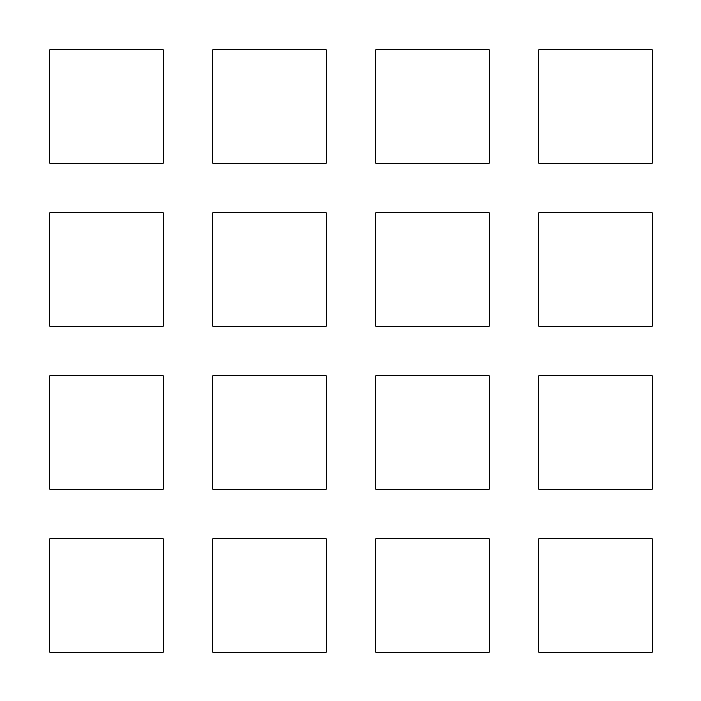
\includegraphics[width=\textwidth]{krunimir/examples/squares}
    \caption{Mřížka čtverců}\label{fig:krunimir-squares}
  \end{subfigure}
  ~
  \begin{subfigure}{0.3\textwidth}
    \centering
    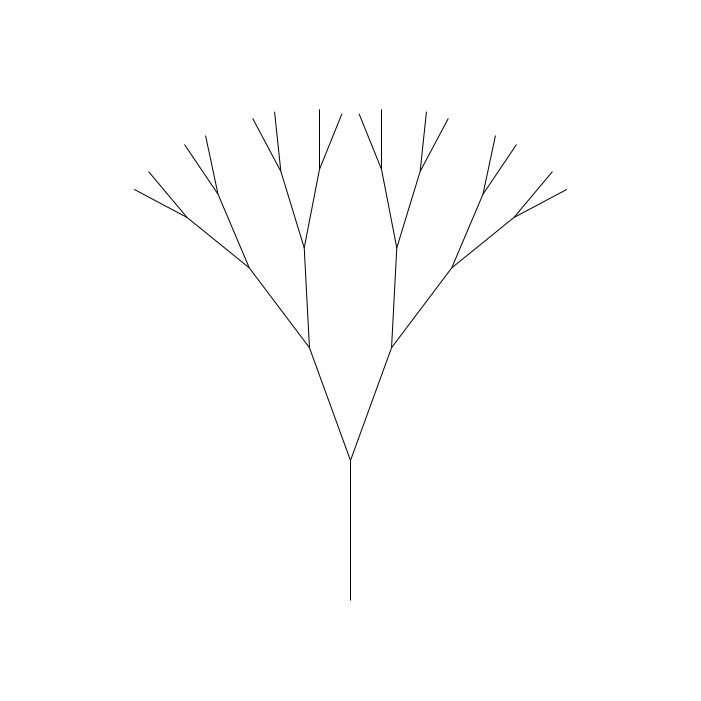
\includegraphics[width=\textwidth]{krunimir/examples/bintree}
    \caption{Binární strom}\label{fig:krunimir-bintree}
  \end{subfigure}

  \caption{Výsledné obrázky z příkladů}
  \protect\label{fig:krunimir-examples}
\end{figure}

\section{Analýza}

Problém si můžeme rozdělit na tři části:

\begin{enumerate}

\item \emph{Syntaktická analýza} (\uv{parsování}) zpracuje vstupní řetězec na
  \emph{abstraktní syntaktický strom}, který zachycuje strukturu programu ve
  formě, která je jednoduše zpracovatelná v dalších fázích.

\item Následuje \emph{vyhodnocení}, kdy ze syntaktického stromu vypočteme
  výslednou stopu (ve vektorové podobě jako seznam úseček).

\item Poslední částí je \emph{vykreslení}, které vykreslí vyhodnocenou stopu do
  obrázku. Budeme exportovat do rastrových obrázků formátu PNG a vektorových
  formátu SVG.

\end{enumerate}

Pomocí tohoto jednoduchého rozdělení můžeme naše řešení rozvrhnout do sedmi
modulů:

\begin{description}

\item @t{Krunimir.Main} exportuje @t{main}, která slouží jako rozhraní s
uživatelem. \footnote{Podobně jako funkce @t{main()} v jazyku C}
  @idx{Krunimir.Main}
  @idx{Krunimir.Main.main}

\item @t{Krunimir.Parser} exportuje funkci @t{parse}, která z textového
zápisu programu vytvoří syntaktický strom (nebo syntaktickou chybu).
  @idx{Krunimir.Parser}
  @idx{Krunimir.Parser.parse}

\item @t{Krunimir.Ast} definuje datové typy, které reprezentují syntaktický
strom.
  @idx{Krunimir.Ast}

\item @t{Krunimir.Evaluator} poskytuje funkci @t{eval}, která ze
syntaktického stromu vypočte výslednou stopu.
  @idx{Krunimir.Evaluator}
  @idx{Krunimir.Evaluator.eval}

\item @t{Krunimir.Trace} definuje datové typy a funkce spojené se stopou želvy.
  @idx{Krunimir.Trace}

\item @t{Krunimir.PngRenderer} exportuje funkci @t{renderPng}, která vykreslí
  stopu jako PNG obrázek.
  @idx{Krunimir.PngRenderer}
  @idx{Krunimir.PngRenderer.renderPng}

\item @t{Krunimir.SvgRenderer} poskytuje funkci @t{renderSvg}, jenž uloží stopu
  ve vektorovém formátu SVG.
  @idx{Krunimir.SvgRenderer}
  @idx{Krunimir.SvgRenderer.renderSvg}

\end{description}

\input{krunimir/Krunimir/Main.lhs}
\input{krunimir/Krunimir/Ast.lhs}
\input{krunimir/Krunimir/Parser.lhs}
\input{krunimir/Krunimir/Trace.lhs}
\input{krunimir/Krunimir/Evaluator.lhs}
\input{krunimir/Krunimir/PngRenderer.lhs}
\input{krunimir/Krunimir/SvgRenderer.lhs}

\printindex

\bibliographystyle{babplain}
\bibliography{bibliography}

\end{document}
